\section{Introduction}
This report will describe, outline and display the efforts made towards creating an autonomous conversational agent (chatbot) to interact with a human user. The primary purpose includes searching the internet for cheap train tickets between two destinations and present the findings to the user to for procurement. This objective should be achieved through a short series of dialogue interactions. The second motive this chatbot aims to realise is the improvement to customer service through conversation. There is no limitation to the depth of assistance the chatbot can provide; a regression model to predict the arrival time at a final station of a journey was designed and implemented. Lastly, the chatbot must have the ability to provide train operators with assistance when dealing with contingencies through several suggested resolution actions. This is achieved by employing a knowledge base (KB) which includes information regarding possible contingencies and regulation documents with actions within accordance.



% (Brief introduction to the coursework. 
% You don't have to write much.  
% You may introduce a bit on chatbot in general if like, and why an intelligent chatbot is useful using the subsections headings if you wish.)  

\subsection{Background and Motivation}
Chatbots are useful tools for improving efficiency and reducing the human labour during tedious tasks. Chatbots in their infancy used predefined rules to converse with humans which led to considerable limitations in communication. However, the succeeding chat-bots utilised machine learning (ML) and natural language processing (NLP) to analyse and respond intelligently with context and nuance to the users input. Section \ref{sec: related works} describes the current standard of chatbots which are free to acquire and use. At present no commercially available chatbot hold the ability to confidently check live train times and prices or accurately predict delayed arrival times. The absence of these abilities is the motivation behind the project with the objective outlined in Section \ref{Sec: Aim and Objs}.


% A bit background information on chatbot in general and the coursework specification \citep{AI2018CW}.

\subsection{Aim and Objectives of this coursework}\label{Sec: Aim and Objs}
% You may rephrase the the aim and objectives from your point of view.
% Due to the limited access to train times and tickets we are poised with the task of: \begin{enumerate}
To successfully realise this project and develop a sufficient working chatbot, the following objectives must be met and accomplished: 
\begin{enumerate}
    \item Create a conversational agent
        \begin{enumerate}
            \item Create code to clean and deconstruct a users input to a manageable format
            \item Create a NLP mechanism to determine the users intention of their input 
            \item Create an interactive Graphical User Interface (GUI) for better experience
        \end{enumerate}

    \item Scrape train time service websites for live train times and prices
        \begin{enumerate}
            \item Accumulate a minimum of 5 online services or websites that can produce accurate live train times and prices
            \item Extract the relevant information into a sufficient data structure
        \end{enumerate}

    \item Display and converse the data collected to the user in a understandable manner
        \begin{enumerate}
            \item Displays the relevant information i.e. website name, fare amount and cheapest fare clickable link. 
        \end{enumerate}

    \item Deploy a deep learning regression network to predict a delay train line's arrival and departure
        \begin{enumerate}
            \item Collect dataset of train journeys from Norwich to London Liverpool Street
            \item Preprocess the data for optimal utilisation when using neural network models
            \item Develop a network model which will efficiently output a numeric value based on the users input
            \item Measure and refine the model until a satisfactory quality has been achieved
            \item Deploy the model using the chat-bot
        \end{enumerate}

    \item Create rule engine (RE) to provide contingency plans
        \begin{enumerate}
            \item Implement NLP technique to extract locations and blockage type from the staff user input. 
            \item The train stations can only be between Colchester and Norwich on Great Eastern Track in Greater Anglia.
            \item Create Rule Engine (RE) to provide alternate plans / routes to the train station staff based on the blockage type and stations provided.
        \end{enumerate}
\end{enumerate}

\subsection{Difficulties and Risks}
This project includes several inherent factors which need to be considered to avoid unethical practises and application restrictions. Firstly, a restriction against the use of paid APIs was established. During the attempted exploration and extraction of data, a large quantity of websites offered access to their data through their API after a paid transaction. The choice to circumvent this option avoid unwanted financial burden and mitigates any economic advantage against colleagues attempting the same project.\vspace{0.5cm}

\noindent
Moreover, web scraping is a topic of ethical consideration and requires a thorough evaluation before commencing an automated scraping script. Due to moral concerns, caution is needed to avoid overloading a website with too many requests in a short space of time. Failure to acknowledge these concerns could overload the server hosting the website, which as a result, could suffer from an overall loss of speed. In an extreme case this can be considered a denial-of-service (DoS) attack. It is common practise to deploy anti-scraping tools on websites which require the user to pass a CAPTCHA before accessing the data. Failure to pass the CAPTCHA will temporarily and on occasion permanently revoke the user access the website.\vspace{0.5cm}

\noindent
Furthermore, online websites can contain personal information that should be avoided by a scraping tool indefinitely. The nature of the data and websites should mitigate any personal information, however caution will be practised to ensure no personal data is extracted. The deployment of artificial ``user-agents'' to access Chrome web browser via Selenium has shown great promise as an option to avoid an accidental security breach of the website and as a result the chat-bot is blocked from said website. However, implementing web scraping scripts employing Selenium requires prior knowledge regarding accessing web elements and locators. Should the website be composed of React element, the challenge of creating dynamic code which searches and extract specific elements becomes too large to become viable. Furthermore, a lot of websites constantly update their locators and web elements, particularly when new features are being deployed as software patches or builds. This periodic shift necessitates a time commitment to maintain a close eye on the automation scripts created to extract data. Because web scraping scripts may begin to malfunction if the locators are altered, resulting in unexpected results displayed on the chatbot's graphical user interface.
 \vspace{0.5cm}

\noindent
The NLP models used in this project which are outlines in Section \ref{Sec: Methods/NLP} demonstrated considerable difficulty in determining small or all UK cities. Hence, the objective to extract locations from the sentences became a largely challenging aspect of this project. In addition to the cities, the indicated date and time were difficult to extract because the pre-trained spaCy models that are now in use are not strong enough to retrieve the information from a lengthy or intricate user input. Therefore, it was necessary to find alternative methods in order to complete the necessary chatbot tasks. \vspace{0.5cm}

\subsection{Work Plan}
The following section will outline what each member's efforts have been focused over the duration of the project.
\subsubsection{Cemal Ata Uzgoren}
\begin{itemize}
    \item Took the poston as team leader
    \item Led the design and development of the GUI for the chatbot
    \item Led the integrity issues handling across the all three NLP tasks (Task A, Task B, Task C)
\end{itemize}
\subsubsection{Aman Seth}
\begin{itemize}
    \item Implemented multiprocessing among six scraper scripts resulting in reduced time consumption in fetching and displaying cheapest fare results on GUI.
    \item Led the NLP implementation at the backend of the chatbot graphical user interface for all three tasks (Task A, Task B, Task C)
    \item Led the embedding of the regression model into the conversational script
    
\end{itemize}
% Aman seth took the lead on embedding the regression model developed into the conversional script.
\subsubsection{Josh Newton}
% The efforts made by Josh included:
\begin{itemize}
    \item Created initial web scraping scripts which included the a method using either the Selenium library or sending a prefilled payload to the service
    \item Led the processing and exploration of the dataset provided for training a regression model to predict the arrival time at Norwich during a journey departing from London Liverpool Street
    \item Led the evaluation of multiple models to conclude the most efficient and practical model to implement.
\end{itemize} 

\subsubsection{Ganttchart}
The following figure displays the planned and executed timeline of events required to complete the aims outlined in Section \ref{Sec: Aim and Objs}.
\begin{figure}[!htbp]
    \centering
    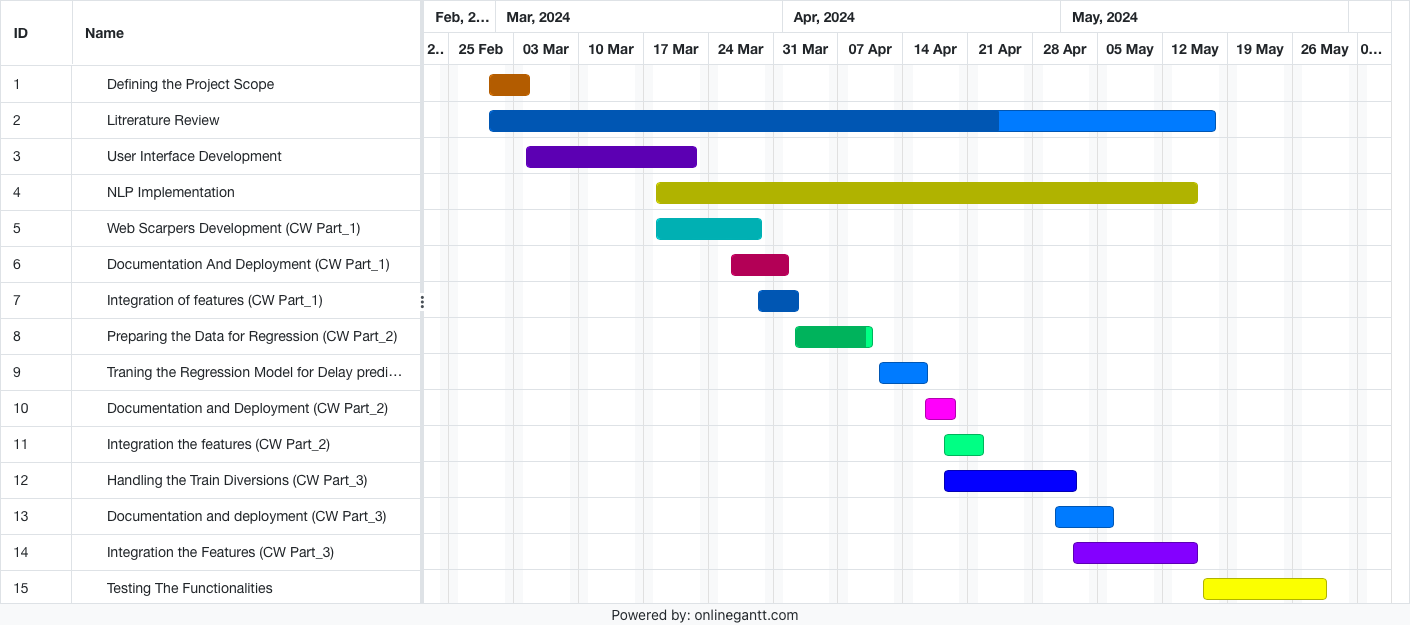
\includegraphics[width=\linewidth]{Diagrams/gant_chart.png}
    \caption{Gantt Chart displaying the execution timeline of tasks}
    \label{Fig: Gantt Chart}
\end{figure}
